\documentclass[12pt,a4paper]{article}
\usepackage{amsmath}
\usepackage{graphicx}

\begin{document}
	
% Folha de rosto
\begin{titlepage}
	\centering
	\vspace{2cm}
	
	{UNIVERSIDADE FEDERAL FLUMINENSE} \\ [0.1cm]
	{BACHARELADO EM CIÊNCIA DA COMPUTAÇÃO} \\ [0.1cm]
	{TCC00349 - AVALIAÇÃO DE DESEMPENHO}
	
	\vfill
	
	{\Large \bfseries Trabalho de simulação utilizando a ferramenta Java Modelling Tools}
	
	\vfill
	
	{BEATRIZ DE OLIVEIRA PIEDADE}
	
	\vfill
	{NITERÓI} \\
	{2024}
\end{titlepage}

% Conteúdo
\newpage
\section{Modelo 1 - M/M/1}

% Métricas do enunciado
\begin{description}
	\item[Tempo médio entre chegadas:] 0.5 u.t, logo $\lambda$ = 2 clientes por u.t.
	\item[Tempo de atendimento do servidor:] E[X] = $\frac{1}{\mu}$ = 0.25 u.t por cliente, logo $\mu$ = 4 clientes por u.t.
	\item[Capacidade:] Ilimitada.
\end{description}

% Print do sistema
\subsection{Topologia do sistema}
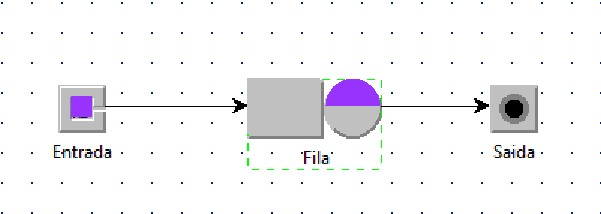
\includegraphics[width=\linewidth]{topologias/m1.jpg}

% Contas
\subsection{Solução analítica}

Fórmula de \(L\):
\begin{equation*}
	\begin{aligned}
		&L = {\lambda} \cdot {W} \\
		&L = {\lambda} \cdot \frac{1}{\mu-\lambda} \\
		&L = {2} \cdot \frac{1}{4-2} \\
		&L = \frac{2}{2} \\
		&L = 1 \\
	\end{aligned}
\end{equation*}

\noindent
\\ 
Fórmula de \(W\):
\begin{equation*}
	\begin{aligned}
		&W = \frac{1}{\mu - \lambda} \\
		&W = \frac{1}{4 - 2} \\
		&W = \frac{1}{2} \\
		&W = {0.5} 
	\end{aligned}
\end{equation*}


\noindent
\\
Fórmula de \(W_Q\):
\begin{equation*}
	\begin{aligned}
		&W_Q = \frac{L_Q}{\lambda} \\
		&W_Q = \frac{\frac{\lambda^2}{\mu \cdot ({\mu - \lambda})}}{\lambda} \\
		&W_Q = \frac{\lambda^2}{\lambda \cdot \mu \cdot ({\mu - \lambda})} \\
		&W_Q = \frac{\lambda}{\mu \cdot ({\mu - \lambda})} \\
		&W_Q = \frac{2}{4 \cdot ({4 - 2})} \\
		&W_Q = \frac{1}{2 \cdot ({2})} \\
		&W_Q = \frac{1}{4} \\
		&W_Q = {0.25}
	\end{aligned}
\end{equation*}

% Métricas do programa
\subsection{Especificação das métricas da simulação}
\begin{description}
	\item[Class:] Entrada 
	\begin{itemize}
		\item $\lambda$: 2
		\item mean: 0.5
	\end{itemize}
	\item[Queue Section:] Fila
	\begin{itemize}
		\item Capacity: Infinite
	\end{itemize}
	\item[Service Section:] Atendimento
	\begin{itemize}
		\item Number of Servers: 1
		\item $\lambda$: 4
		\item mean: 0.25
	\end{itemize}
	\item[Performance Indices:] Valores a simular 
	\begin{itemize}
		\item Number of customers
		\item Response Time
		\item Queue Time
	\end{itemize}
\end{description}

% Conclusão
\subsection{Comparação}

\begin{table}[h]
	\centering
	\begin{tabular}{|l|l|l|} 
		\hline
		\textbf{Métrica} & \textbf{Solução analítica} & \textbf{Valor simulado} \\ 
		\hline
		Number of customers \((L)\) & 1 & 1.0219 \\
		\hline
		Response Time \((W)\) & 0.5 & 0.5066 \\
		\hline
		Queue Time \((W_Q)\) & 0.25 & 0.2535 \\
		\hline
	\end{tabular}
\end{table}

\newpage
\section{Modelo 2 - M/M/1/10}

% Métricas do enunciado
\begin{description}
	\item[Tempo médio entre chegadas:] 0.5 u.t, logo $\lambda$ = 2 clientes por u.t.
	\item[Tempo de atendimento do servidor:] E[X] = $\frac{1}{\mu}$ = 0.35 u.t por cliente, logo $\mu$ = 2.857 clientes por u.t.
	\item[Capacidade:] Limitada a K = 10 clientes (1 cliente atendido e 9 na fila).
\end{description}

% Print do sistema
\subsection{Topologia do sistema}
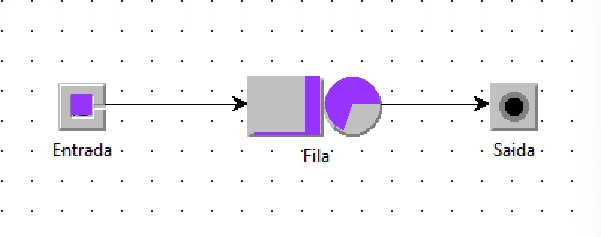
\includegraphics[width=\linewidth]{topologias/m2.jpg}

% Contas
\subsection{Solução analítica}

Fórmula de \(L\):
\begin{equation*}
	\begin{aligned}
		&L = \frac{\rho}{1 - \rho} - \frac{(K + 1) \cdot \rho^{K+1}}{1 - \rho^{K+1}} \\
		&L = \frac{\frac{\lambda}{\mu}}{1 - \frac{\lambda}{\mu}} - \frac{(K + 1) \cdot \frac{\lambda}{\mu}^{K+1}}{1 - \frac{\lambda}{\mu}^{K+1}} \\
		&L = \frac{\frac{2}{2.857}}{1 - \frac{2}{2.857}} - \frac{(10 + 1) \cdot \frac{2}{2.857}^{10+1}}{1 - \frac{2}{2.857}^{10+1}} \\
		&L = \frac{0.7}{1 - 0.7} - \frac{11 \cdot 0.7^{11}}{1 - 0.7^{11}} \\
		&L = \frac{0.7}{0.3} - \frac{11 \cdot 0.019}{1 - 0.019} \\
		&L = 2.333 - \frac{0.209}{0.981} \\
		&L = 2.333 - 0.213 \\
		&L = {2,12}
	\end{aligned}
\end{equation*}


\noindent
\\
Fórmula de \(W\):
\begin{equation*}
	\begin{aligned}
		&W = \frac{L}{\lambda} \\
		&W = \frac{2.12}{2} \\
		&W = {1.06} 
	\end{aligned}
\end{equation*}

% Métricas do programa
\subsection{Especificação das métricas da simulação}
\begin{description}
	\item[Class:] Entrada 
	\begin{itemize}
		\item $\lambda$: 2
		\item mean: 0.5
	\end{itemize}
	\item[Queue Section:] Fila
	\begin{itemize}
		\item Capacity: Finite 10
	\end{itemize}
	\item[Service Section:] Atendimento
	\begin{itemize}
		\item Number of Servers: 1
		\item $\lambda$: 2.857
		\item mean: 0.35
	\end{itemize}
	\item[Performance Indices:] Valores a simular 
	\begin{itemize}
		\item Number of customers
		\item Response Time
		\item Queue Time
		\item Drop Rate
	\end{itemize}
\end{description}

% Conclusão
\subsection{Comparação}

\begin{table}[h]
	\centering
	\begin{tabular}{|l|l|l|} 
		\hline
		\textbf{Métrica} & \textbf{Solução analítica} & \textbf{Valor simulado} \\ 
		\hline
		Number of customers \((L)\) & 2.12 & 2.1456 \\
		\hline
		Response Time \((W)\) & 1.06 & 1.0795 \\
		\hline
		Queue Time \((W_{Q})\) & - & 0.7279 \\
		\hline
		Drop Rate & - & 0.0174 \\
		\hline
	\end{tabular}
\end{table}

\newpage
\section{Modelo 3 - M/M/5}
% Métricas do enunciado
\begin{description}
	\item[Tempo médio entre chegadas:] 0.25 u.t, logo $\lambda$ = 4 clientes por u.t.
	\item[Tempo de atendimento do servidor:] E[X] = $\frac{1}{\mu}$ = 1 u.t por cliente, logo $\mu$ = 1 cliente por u.t.
	\item[Capacidade:] Ilimitada.
\end{description}

% Print do sistema
\subsection{Topologia do sistema}
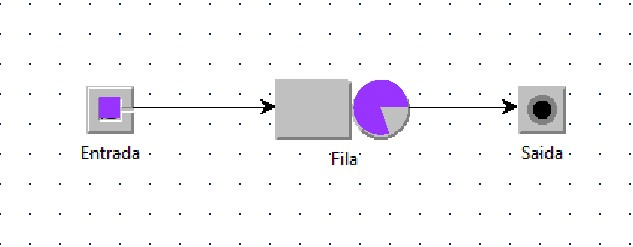
\includegraphics[width=\linewidth]{topologias/m3.jpg}

\subsection{Especificação das métricas da simulação}
\begin{description}
	\item[Class:] Entrada 
	\begin{itemize}
		\item $\lambda$: 4
		\item mean: 0.25
	\end{itemize}
	\item[Queue Section:] Fila
	\begin{itemize}
		\item Capacity: Infinite
	\end{itemize}
	\item[Service Section:] Atendimento
	\begin{itemize}
		\item Number of Servers: 5
		\item $\lambda$: 1
		\item mean: 1
	\end{itemize}
	\item[Performance Indices:] Valores a simular 
	\begin{itemize}
		\item Number of customers
		\item Response Time
		\item Queue Time
	\end{itemize}
\end{description}

\subsection{Comparação}

\begin{table}[h]
	\centering
	\begin{tabular}{|l|l|l|} 
		\hline
		\textbf{Métrica} & \textbf{Solução analítica} & \textbf{Valor simulado} \\ 
		\hline
		Number of customers \((L)\) & - & 6.2073 \\
		\hline
		Response Time \((W)\) & - & 1.5519 \\
		\hline
		Queue Time \((W_{Q})\) & - & 0.5499 \\
		\hline
	\end{tabular}
\end{table}

\newpage
\section{Modelo 4 - M/M/1 $\rightarrow$ M/M/1}

% Métricas do enunciado
\begin{description}
	\item[Tempo médio entre chegadas:] 0.5 u.t, logo $\lambda$ = 2 clientes por u.t.
	\item[Tempo de atendimento do servidor 1:] E[X] = $\frac{1}{\mu}$ = $\frac{1}{3}$ u.t por cliente, logo $\mu$ = 3 clientes por u.t.
	\item[Tempo de atendimento do servidor 2:] E[X] = $\frac{1}{\mu}$ = 0.25 u.t por cliente, logo $\mu$ = 4 clientes por u.t.
	\item[Capacidade:] Ilimitada.
\end{description}

% Print do sistema
\subsection{Topologia do sistema}
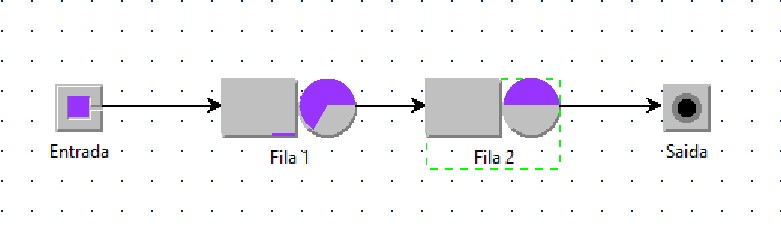
\includegraphics[width=\linewidth]{topologias/m4.jpg}

% Contas
\subsection{Solução analítica}

\noindent
\\
Fórmula de \(L_{1}\):
\begin{equation*}
	\begin{aligned}
		&L_{1} = \lambda_{inicial} \cdot {E[W]_{1}} \\
		&L_{1} = {\lambda_{inicial}} \cdot \frac{E[X]_{1}}{1-{\lambda_{inicial}}\cdot{E[X]_{1}}} \\
		&L_{1} = {2} \cdot \frac{\frac{1}{3}}{1-{2}\cdot{\frac{1}{3}}} \\
		&L_{1} = {2} \cdot \frac{0.333}{1-{2}\cdot{0.333}} \\
		&L_{1} = \frac{0.666}{1-0.666} \\
		&L_{1} = \frac{0.666}{0.334} \\
		&L_{1} = 1.994 \\
	\end{aligned}
\end{equation*}

\noindent
\\
Fórmula de \(L_{2}\):
\begin{equation*}
	\begin{aligned}
		&L_{2} = \lambda_{1} \cdot {E[W]_{2}} \\
		&L_{2} = {\lambda_{1}} \cdot \frac{E[X]_{2}}{1-{\lambda_{1}}\cdot{E[X]_{2}}} \\
		&L_{2} = {2} \cdot \frac{0.25}{1-{2}\cdot{0.25}} \\
		&L_{2} = \frac{0.5}{1-0.5} \\
		&L_{2} = \frac{0.5}{0.5} \\
		&L_{2} = 1 \\
	\end{aligned}
\end{equation*}

\noindent
\\
Fórmula de \(L_{sistema}\):
\begin{equation*}
	\begin{aligned}
		&L_{sistema} = L_{1} + L_{2} \\
		&L_{sistema} = 1.994 + 1 \\
		&L_{sistema} = 2.994 \\
	\end{aligned}
\end{equation*}

\noindent
\\
Fórmula de \(W_{1}\):
\begin{equation*}
	\begin{aligned}
		&W_{1} = \frac{L_{1}}{\lambda_{inicial}} \\
		&W_{1} = \frac{1.994}{2} \\
		&W_{1} = 0.997
	\end{aligned}
\end{equation*}

\noindent
\\
Fórmula de \(W_{2}\):
\begin{equation*}
	\begin{aligned}
		&W_{2} = \frac{L_{2}}{\lambda_{1}} \\
		&W_{2} = \frac{1}{2} \\
		&W_{2} = 0.5
	\end{aligned}
\end{equation*}

\noindent
\\
Fórmula de \(W_{sistema}\):
\begin{equation*}
	\begin{aligned}
		&W_{sistema} = W_{1} + W_{2} \\
		&W_{sistema} = 0.997 + 0.5 \\
		&W_{sistema} = 1.497
	\end{aligned}
\end{equation*}


% Métricas do programa
\subsection{Especificação das métricas da simulação}
\begin{description}
	\item[Class:] Entrada 
	\begin{itemize}
		\item $\lambda$: 2
		\item mean: 0.5
	\end{itemize}
	\item[Queue Section:] Fila 1
	\begin{itemize}
		\item Capacity: Infinite
	\end{itemize}
	\item[Service Section:] Atendimento da fila 1
	\begin{itemize}
		\item Number of Servers: 1
		\item $\lambda$: 3
		\item mean: 1/3
	\end{itemize}
	\item[Queue Section:] Fila 2
	\begin{itemize}
		\item Capacity: Infinite
	\end{itemize}
	\item[Service Section:] Atendimento da fila 2
	\begin{itemize}
		\item Number of Servers: 1
		\item $\lambda$: 4 
		\item mean: 0.25
	\end{itemize}
	\item[Performance Indices:] Valores a simular 
	\begin{itemize}
		\item Number of customers
		\item Response Time
	\end{itemize}
\end{description}

% Conclusão
\subsection{Comparação}

\begin{table}[h]
	\centering
	\begin{tabular}{|l|l|l|} 
		\hline
		\textbf{Métrica} & \textbf{Solução analítica} & \textbf{Valor simulado} \\ 
		\hline
		Number of customers \((L)\) & 2.994 &  2.9770 \\
		\hline
		Response Time \((W)\) & 1.497 & 1.4919 \\
		\hline
	\end{tabular}
\end{table}

\end{document}
